\documentclass[a4paper, titlepage]{jsarticle}

\date{\today}
\usepackage[dvipdfmx]{graphicx}
\usepackage{url}
% \usepackage[T1]{fontenc}
\usepackage{float}
\usepackage{ascmac}
\usepackage{pdfpages}

\title{ドローン宅配事業者支援システム}

\author{土佐山田IT株式会社 \and
        久保田 天治 \and 塩澤 康志 \and 蝉 祐介 \and 寺内 俊輔 \and 林 晃太郎 \and 松本 吏司}

\begin{document}
\maketitle

\tableofcontents

\clearpage

\section{現状の課題}
2022年日本における宅配便取扱個数は50億個を超えた.
忙しい日常がある中で,商品や郵便物を手軽に送受できる宅配便は多くの人々にとって頼りにされ,図\ref{fig:home_delivery}のように宅配需要は増加し続けている.
特に新型コロナウイルスの影響により,オンラインショッピングの増加や非接触配達の需要が高まり,宅配業界は一層の成長を遂げた.

しかし,宅配サービスの拡大と需要増加には新たな課題も浮かび上がっている,最も顕著な課題は宅配業界における労働力不足だ.
図\ref{fig:working_population}のように少子高齢化社会に伴う労働人口の減少により,現状の宅配サービスを維持することは日々困難になっている.
特に過疎地域や離島においては,現状の輸送方法では効率が悪く輸送方法の効率化が求められる.
\begin{figure}[H]
    \centering
    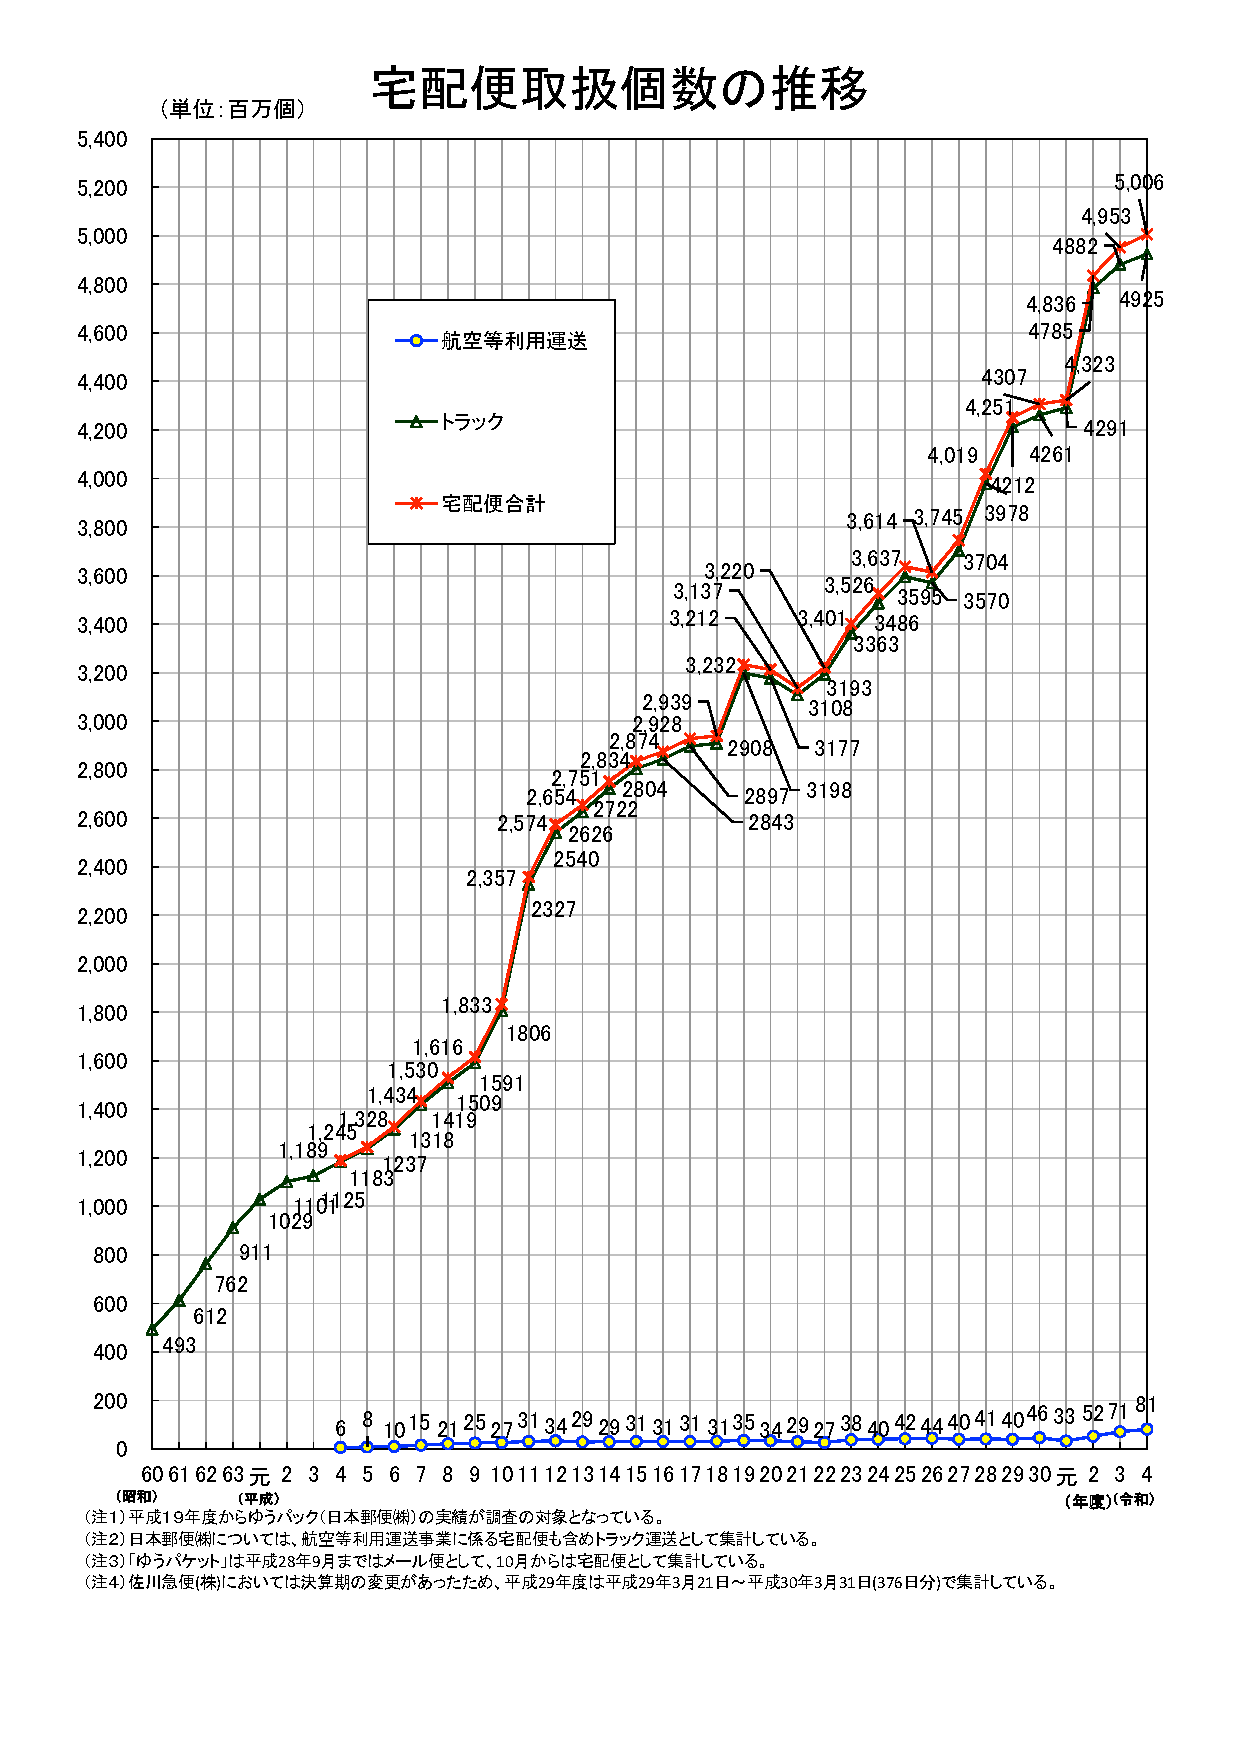
\includegraphics[width=0.6\textwidth]{./home_delivery.pdf}
    \caption{宅配便取扱個数の推移:\cite{home_delivery_2022}より引用}
    \label{fig:home_delivery}
\end{figure}
\begin{figure}[H]
    \centering
    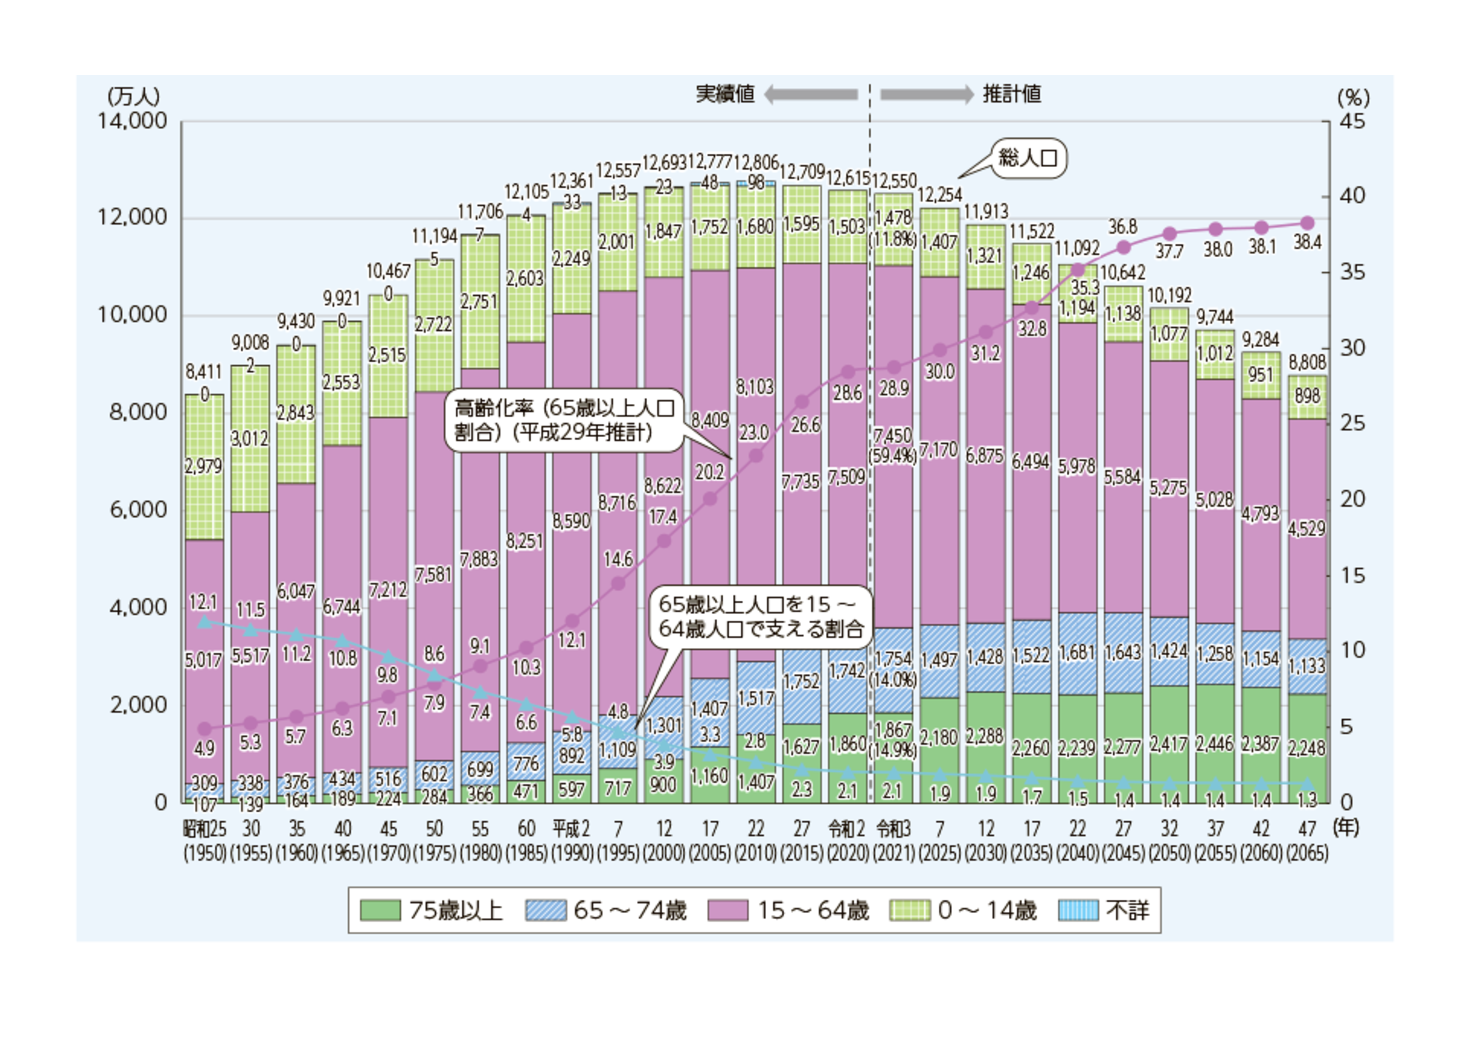
\includegraphics[width=0.8\textwidth]{./working_population.pdf}
    \caption{労働人口の減少:\cite{working_population_2022}より引用}
    \label{fig:working_population}
\end{figure}

\section{課題解決のための提案}
上記の課題を解決するため,効率的かつ人手不足を解消できるようなドローン宅配事業者支援システムを提案する.
このシステムによる課題の解決方法を以下に示す.
\begin{itemize}
    \item ドローンの操縦を自動化することで,より少ない人手で大量の荷物を個人宅に運搬でき,
    労働力不足の問題に対処できる.従来の宅配サービスと比較して労働者への依存度が低くなり,配送コスト削減と労働環境の改善に期待できる.

    \item 離島や過疎地域など従来の方法では配送コストが高かった地域にも,効率的に配送を行うことができる.
    これによりこれらの地域においても高速かつ手頃値段の宅配サービスが提供され,地域経済の活性化が促進できる.

    \item ドローン宅配事業者の支援システムは,多くの事業者に提供され新規ドローン宅配事業者の参入を奨励できる.
    新規ドローン宅配事業者の参入に伴う宅配業務従事者の増加と競争の活発化は,労働力不足の解消,サービス品質の向上,価格競争力の向上につながり,消費者にとって選択肢が増えることで市場が活性化する.

    \item 多くのドローン宅配事業者が共通の支援システムを使用することで,スケールメリットを最大限に活用しコスト削減を実現できる.
    経済的なメリットは宅配業界全体に波及し,より効率的なサービス提供が可能になる.

    % 本筋から外れるためコメントアウト
    % \item ドローン宅配は過疎地域の経済を支え,郊外地域に新たなビジネス機会を提供する.
    % 地域社会の発展に寄与し,地方経済を活性化させるポテンシャルがある.

    % \item 環境への負荷を軽減する.電動または電池駆動のドローンを使用することで,排ガス排出が削減され,環境への負荷が低減する.これは環境への配慮を重視する現代社会に貢献できる.
\end{itemize}

\section{機能の概要・前提条件・制約事項}
\subsection{機能概要}
本システムは管理者,ドローン宅配事業者,使用者が存在する.それぞれに向けた機能の概要を説明する.
\subsubsection{管理者向け機能}
\begin{itemize}
    \item ログインログアウト機能
    \item 会員管理機能
    \item ドローン宅配事業者会員登録承認機能
    \item 会員情報閲覧機能
    \item 利用情報分析機能
    \item 宅配依頼受付機能
    \item 宅配仕事割り振り機能
    \item ドローン貸出機能
    \item 貸出ドローン情報管理機能
\end{itemize}
\subsubsection{ドローン宅配事業者向け機能}
\begin{itemize}
    \item ログインログアウト機能
    \item ドローン宅配事業者会員登録申請
    \item 宅配依頼承諾機能
    \item 配達完了通知機能
    \item 宅配場所登録機能
    \item ドローンレンタル機能
    \item 退会機能
\end{itemize}
\subsubsection{使用者向け機能}
\begin{itemize}
    \item ログインログアウト機能
    \item 使用者会員登録機能
    \item 宅配依頼機能
    \item 宅配場所登録機能
    \item 退会機能
\end{itemize}
\subsection{前提条件}
\begin{itemize}
	\item 宅配元と宅配先がお互いドローン着地地点を登録している
	\item ドローン宅配事業者は搬送装置を無人航空機の登録制度に基づき国土交通省のシステムに登録すること
	\item 利用者は日本語を理解できること
\end{itemize}
\subsection{制約条件}
\begin{itemize}
	\item 利用者が情報を登録するときに虚偽の情報を登録しないこと
	\item 管理者は利用者の情報を本システムの利用目的以外で使用しないこと
	\item 管理者は利用者の個人情報の管理を情報漏洩のないように行うこと
	\item ドローン宅配事業者は航空法施行規則236条に基づき搬送装置の適切な運用を行うこと
	\item 利用者は利用規約を順守すること
\end{itemize}
\section{情報・金銭の流れ}

\subsection{情報の流れ}
本システムにおける情報の流れを図\ref{fig:info_flow_1}に示す.
本システムは,利用者(送り主及び受け取り主)が使用する端末,ドローン宅配事業者が利用する端末,システム管理者が利用する端末及び,システム中核を担うサーバとデータベースによって構成される.

各ユーザからの要求を受けサーバが処理を行い,webページやアプリケーションに適した情報を提供する.

\begin{figure}[H]
  \centering
  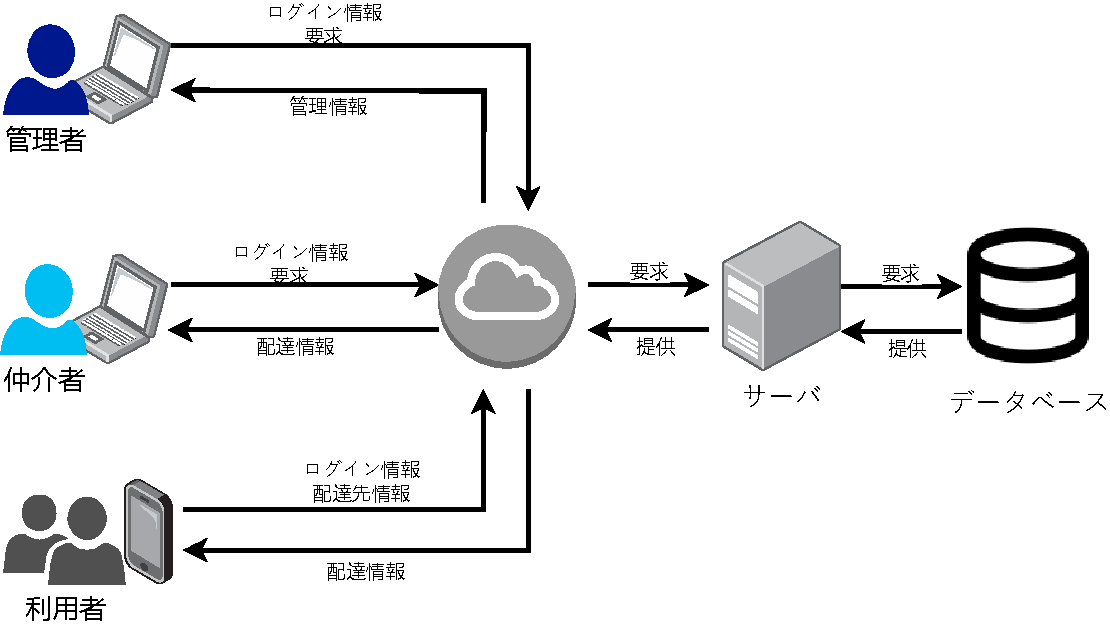
\includegraphics[width=0.6\linewidth]{./info_flow.pdf}
  \caption{本システムにおける情報の流れ}
  \label{fig:info_flow_1}
\end{figure}

\subsection{金銭の流れ}
本システムにおける金銭の流れを図\ref{fig:money_flow_1}に示す.

\begin{figure}[H]
  \centering
  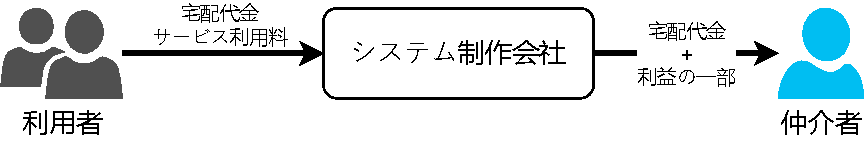
\includegraphics[width=0.6\linewidth]{./money_flow.pdf}
  \caption{本システムにおける金銭の流れ}
  \label{fig:money_flow_1}
\end{figure}


\section{想定する利用者}
本システムが想定する利用者を下記に示す.
\begin{itemize}
        \item 荷物の送受を希望する事業者または個人
        \item ドローン宅配事業者
\end{itemize}

\section{運用・保守}

\section{ハードウェア・ソフトウェアの構成}
\subsection{ハードウェア構成}
本システムのハードウェア構成を表\ref{fig:hardware}に示す.
\begin{table}[H]
 \begin{center}
  \caption{ハードウェアの構成}
    \label{fig:hardware}
  \begin{tabular}{ccc} \hline
    項目 & 種類 & 数量 \\ \hline \hline
    メインサーバ & レンタルサーバ & 2 \\
    データベースサーバ & レンタルサーバ & 2 \\
    管理者端末 & PC & 1 \\
    ドローン宅配事業者端末 & PC & ドローン宅配事業者数 \\
    利用者端末 & スマートフォン & 利用者数 \\
    搬送装置 & ドローン & ドローン宅配事業者希望数以上 \\ \hline
  \end{tabular}
 \end{center}
\end{table}
\subsection{ソフトウェア構成}
本システムのソフトウェア構成を表\ref{fig:software}に示す.
\begin{table}[H]
 \begin{center}
  \caption{ソフトウェアの構成}
    \label{fig:software}
  \begin{tabular}{cc} \hline
    項目 & ソフトウェア \\ \hline \hline
    Webサーバ & 未定 \\
    データベース管理システム & 未定 \\
    管理者端末 & Linux系OS \\
    ドローン宅配事業者端末 & 未定 \\
    利用者端末 & Android,iOS \\
    搬送装置 & 未定 \\ \hline
  \end{tabular}
 \end{center}
\end{table}

\section{費用・効果}
\subsection{システムの効果}
本システムを導入することによって,ドローンを用いた無人宅配が可能となり,宅配サービスの人手不足を解消することができると考えられる.また,これから先進するであろうリモート診療に利用できると考えられる.

\subsection{収益}
本システムの収益は配達による収入を想定している.配送料を600円,1日に配達する荷物の数を,宅配便の1日当たりの荷物数の約0.14\%の20,000個とすると5年間の配達による収入は
\begin{center}
    600円×20,000個×30日×60ヶ月=21,600,000,000円
\end{center}
となる.

\subsection{システムの導入・運用コスト}
本システムの導入コストは表1,運用コストは表2のようになる.
\begin{table}[htbp]
    \centering
    \begin{tabular}{c c c c c}
    \hline
    項目 & 単価(円) & 数量 & 金額(円) & 備考 \\
    \hline \hline
    物流ドローン(貸出用) & 3,000,000 & 200台 & 600,000,000 &  \\
    サーバ(レンタル) & 2,000 & 4ヶ月×2台 & 16,000 & \\
    システム設計人件費 & 40,000 & 38日×2人 & 3,040,000 & \\
    システム実装人件費 & 40,000 & 34日×6人 & 8,160,000 & \\
    \hline \hline
     & 合計 &  & 612,736,000 &  \\
    \hline
    \end{tabular}
    \caption{導入コスト}
    \label{tab:label1}
\end{table}

\begin{table}[htbp]
    \centering
    \begin{tabular}{c c c c c}
    \hline
    項目 & 単価(円) & 数量 & 金額(円) & 備考 \\
    \hline \hline
    サーバ(レンタル) & 2,000 & 60ヶ月×2台 & 240,000 & 12ヶ月×5年×1台 \\
    維持費用 & 612,736,000 & 5年 & 306,368,000 & (導入コスト×10\% )×5年 \\
    宅配事業者報酬 & 150 & 20,000個×30日×60ヶ月 & 5,400,000,000 & 報酬×1日当たりの荷物の数×日数 \\
    中間配送費用 & 35000 & 40台×30日×60ヶ月 & 2,520,000,000 & 1台あたりの報酬×台数×日数 \\
    \hline \hline
     & 合計 &  & 8,226,608,000 &  \\
    \hline
    \end{tabular}
    \caption{運用コスト}
    \label{tab:label2}
\end{table}

上記を踏まえて,システムの開発と5年間の運用にかかる費用は次のようになる.
\begin{center}
    612,736,000円(導入コスト)+8,226,608,000円(運用コスト)=8,839,344,000円
\end{center}

\subsection{利益}
本システムを5年間運用した際の利益は以下のようになる.
\begin{center}
    21,600,000,000円(収益)-8,839,344,000(費用)=12,760,656,000円
\end{center}

\section{開発体制と工程計画}
本システムの開発は土佐山田IT株式会社の6名により実装する.

本システムの工程計画は図\ref{schedule}に示す.
\begin{figure}[htbp]
        \label{schedule}
        \centering
        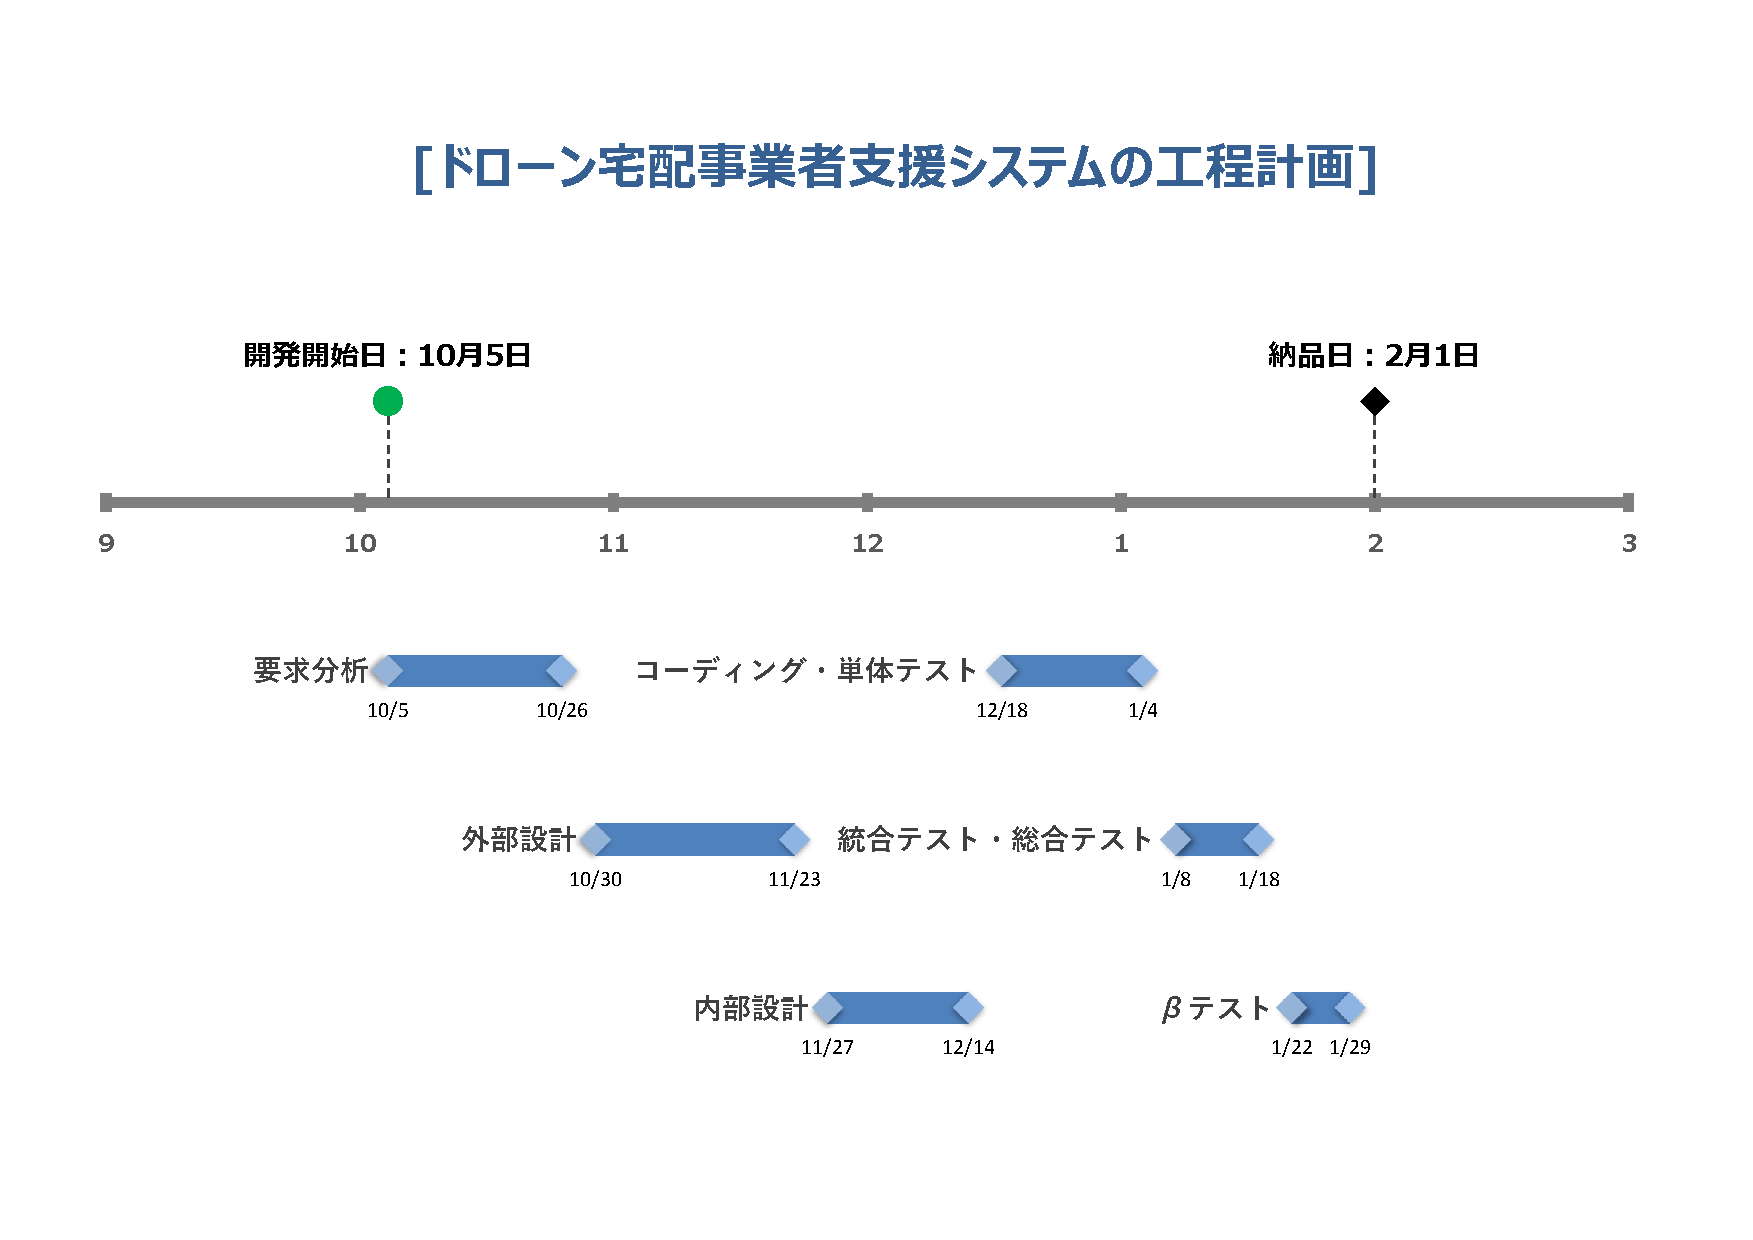
\includegraphics[width=15cm]{schedule.pdf}
        \caption{工程計画}
\end{figure}

\section{本システムのアピールポイント}
\begin{enumerate}
        \item 未だに日本に存在のしないシステムである.
        \item 22年度の宅配荷物数は50億個であり,8年連続史上最高を更新中である.しかし,人手不足が深刻化しており,この課題の解決策のひとつとなりうる.
        \item 交通渋滞や地理的な制約を受けずに荷物を迅速かつ効率的に配達することが可能である.
        \item 災害時などで交通インフラが破壊されたとしても物理的障害の影響が少ないため,必要な物資や医療用品の迅速な配達が可能である.
        \item 離島や山間部などのアクセスが難しい地域において従来の宅配方法と比較し,大幅なコスト削減になる.
        \item 今日リモート診療が普及し始めている.リモート診療とドローン宅配を併用すると患者は外出する必要がなくなるため,感染リスクを極力減らすことができる.
\end{enumerate}

\section{貢献度}
システム提案書では各メンバーが以下を担当した.
\begin{enumerate}
    \item 1240312 久保田 天治: 機能の概要・前提条件・制約事項一部,ハードウェアとソフトウェアの構成
    \item 1250329 塩澤 康志: 費用・効果
    \item 1250333 蝉 祐介: 運用・保守
    \item 1250348 寺内 俊輔: 機能の概要・前提条件・制約事項一部,現状の課題,課題解決のための提案,全体の枠組み,全体の統合
    \item 1250358 林 晃太郎: 想定する利用者,スケジュール,本システムのアピールポイント
    \item 1250371 松本 吏司: 情報・金銭の流れ,全体の枠組み
\end{enumerate}

\bibliography{References.bib}
\bibliographystyle{plain}


\end{document}